%!TEX encoding = UTF-8 Unicode
%!TEX root = ../lect-w12.tex

%%%
\Subsection{Projekt: \texttt{music}}
\begin{Slide}{Projekt: \texttt{music}}\SlideFontSmall
Övergripande syfte:
\begin{itemize}
\item Träna på case-klasser, matchning, saknade värden med \code{Option}, undantag med \code{Try}.
\item Träna på att förstå en modell av en domän som är representerad i kod
\end{itemize}

Innehåll:
\begin{itemize}
\item Skapa, behandla och spela toner och ackord på stränginstrument.
\item Spela toner och ackord med den givna klassen \code{Synth} som erbjuder ett api som gör det enkelt att använda MIDI-synthesizern i JDK8.
\end{itemize}

Förberedelser:
\begin{itemize}
  \item Gör övningen så du har koll på veckans begrepp.
  \item Läs noga igenom domänbeskrivningen och säkerställ att du förstår modellen som beskrivs av den givna koden.
  \item Kolla så den datorn du ska redovisa på kan spela toner. (Det går att göra labben utan ljud men då kanske du ska välja lite andra extrauppgifter, tex rita ut gitarrackord el. liknande)
  \item Ta gärna med lurar som passar i 3,5mm hörlursuttag så du inte stör andra när du labbar i datorsal.
\end{itemize}

\end{Slide}


\begin{Slide}{Modell av toner och ackord}

\begin{itemize}
\item En ton (tonhöjd) representeras med ett heltal.
\begin{Code}
case class Pitch(nbr: Int)
\end{Code}

\item[]

\item Ett ackord är en sekvens av toner (tonhöjder).
\begin{Code}
case class Chord(ps: Vector[Pitch])
\end{Code}
\end{itemize}

\end{Slide}


\begin{Slide}{Domänmodell: Toner, oktaver och ackord}\SlideFontSmall
\begin{itemize}
\item
Inom musiken utgår man från 12 olika \Emph{tonklasser} \Eng{pitch classes}.

\item Dessa tonklasser är ordnade i en sekvens av s.k. \Emph{halva tonsteg} och har följande \Alert{tonklassnamn}:
\begin{Code}
  val pitchClassNames: Vector[String] =
    Vector("C","C#","D","D#","E","F","F#","G","G#","A","A#","B")
\end{Code}
\item Efter tonklassen med namnet \code{B} återkommer tonklassen med namnet \code{C}. (Jämför med vita och svarta tangenter på ett piano.)
\item Symbolen \code{#} uttalas \emph{iss} representerar en höjning ett halvt tonsteg.
%\item Tonklassen \code{C#} uttalas \emph{siss} på svenska, och \emph{see sharp} på engelska.
\item Notera att det är ett halvt tonsteg mellan \code{E} och \code{F}, samt mellan \code{B} och \code{C}.
\item En \Emph{tonklass} \code{(0 until 12)} motsvaras av index i \code{pitchClassNames}.
\item Case-klassen  \code{Pitch(nbr: Int)} representerar \Emph{tonhöjd} där \code{nbr} är i intervallet \code{(0 until 128)} och tillhör tonklassen \code{nbr % 12}.
\item Med heltalsdivision \code{nbr / 12} beräknas tonhöjdens s.k. \Alert{oktav}.
\item En tonhöjd namnges med tonklassnamnet+oktaven, t.ex. \code{"C5"}.

\item Ett \Emph{ackord} består av flera toner som spelas tillsammans.
\end{itemize}
\end{Slide}




\begin{Slide}{Toner på ett stränginstrument}
\begin{minipage}{0.5\textwidth}
\begin{itemize}\SlideFontSmall
\item Gitarr och ukulele har 6 resp. 4 strängar och en greppbräda med s.k. band.

\item Om man trycker ned ett finger på (egentligen bakom) första bandet höjs tonen ett halvt tonsteg.

\item Exempel: om en sträng är stämd i D3 blir tonen om man trycker ned fingret på fjärde bandet F\#3.

\item \href{http://www.gitarr.org}{www.gitarr.org}

\end{itemize}
\end{minipage}
\begin{minipage}{0.45\textwidth}
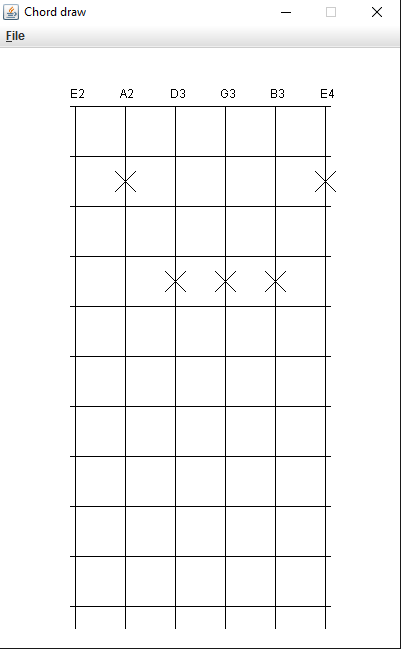
\includegraphics[width=1.0\textwidth]{../img/chords/ChordDraw}
\end{minipage}

\end{Slide}

\begin{Slide}{Modell av tonhöjd}
\begin{CodeSmall}
case class Pitch(nbr: Int) {

  assert((0 to 127) contains nbr, s"Error: nbr $nbr outside (0 to 127)")

  def pitchClass: Int        = nbr % 12

  def pitchClassName: String = ???

  def name: String           = ???

  def octave: Int            = nbr / 12

  def +(offset: Int): Pitch  = Pitch(nbr + offset)

  override def toString      = s"Pitch($name)"
}

object Pitch {

  def fromString(s: String): Option[Pitch] = ???

  def apply(s: String): Pitch = ???
}
\end{CodeSmall}
\SlideFontTiny
Se implementationer här:
\url{https://github.com/lunduniversity/introprog/blob/master/workspace/w10_music/src/main/scala/music/Pitch.scala}
\end{Slide}

\begin{Slide}{Modell av ackord}
\begin{CodeSmall}
case class Chord(ps: Vector[Pitch]) {

  assert(ps.nonEmpty, "Chord pitch sequence is empty")

  val pitchClasses: Vector[Int]   = ps.map(_.pitchClass).toVector

  def apply(i: Int): Pitch = ps(i)

  def intervals(root: Pitch = ps(0)): Vector[Int] = ps.map(_.nbr - root.nbr)

  def relativePitchClasses(root: Pitch = ps(0)): Vector[Int] = ???

  def name(root: Pitch = ps(0)): String = ???

  override def toString = ps.map(_.name).mkString("Chord(",",",")")
}

object Chord {
  def apply(xs: String*): Chord = Chord(xs.map(Pitch.apply).toVector)

  def random(pitchNumbers: Seq[Int] = (60 to 72), n: Int = 3): Chord = ???
}
\end{CodeSmall}
\SlideFontTiny
Se implementationer här:
\url{https://github.com/lunduniversity/introprog/blob/master/workspace/w10_music/src/main/scala/music/Chord.scala}
\end{Slide}

\begin{Slide}{Typhierarki: modell av stränginstrument}\SlideFontSmall
\vspace{-0.5em}\begin{center}
\newcommand{\TextBox}[1]{\raisebox{0pt}[1em][0.5em]{#1}}
\tikzstyle{umlclass}=[rectangle, draw=black,  thick, anchor=north, text width=3cm, rectangle split, rectangle split parts = 3]
\begin{tikzpicture}[inner sep=0.5em, scale=0.9, every node/.style={scale=0.9}]

\node [umlclass, rectangle split parts = 2, xshift=-3cm, text width=5cm] (BaseType)  {
            \textit{\textbf{\centerline{\TextBox{\code{StringInstrument}}}}}
            \nodepart[]{second}
            \TextBox{\code{def toChordOpt: Option[Chord]}}%\vspace{-0.25em}\newline
            %\TextBox{\code{def tuning: Vector[String]}}\vspace{-0.25em}\newline
            %\TextBox{\code{def grip: Vector[Int]}}\vspace{-0.25em}\newline
        };

\pause

\node [umlclass, rectangle split parts = 2, text width=3.9cm] at (-5.2cm,-2.5cm) (Piano) {
            \textbf{\centerline{\TextBox{\code{Piano}}}}
            \nodepart[]{second}
            \TextBox{\code{val isKeyDOwn: Set[Int]}}
        };

\draw[umlarrow] (Piano.north) -- ++(0,0.5) -| (BaseType.south);


\pause



\node [umlclass, rectangle split parts = 2, xshift=0cm, text width=4.5cm] at (0cm,-2.2cm)  (Fretted)  {
            \textit{\textbf{\centerline{\TextBox{\code{FrettedInstrument}}}}}
            \nodepart[]{second}
            \TextBox{\code{def nbrOfStrings: Int}}\vspace{-0.25em}\newline
            \TextBox{\code{def tuning: Vector[Pitch]}}\vspace{-0.25em}\newline
            \TextBox{\code{def grip:   Vector[Int]}}\vspace{-0.25em}\newline
        };

\draw[umlarrow] (Fretted.north) -- ++(0,0.2) -| (BaseType.south);

\pause

\node [umlclass, rectangle split parts = 2, text width=6.1cm]  at (2.2cm,-5.7cm) (Guitar) {
            \textbf{\centerline{\TextBox{\code{Guitar}}}}
            \nodepart[]{second} \TextBox{\footnotesize\code{val pos: (Int,Int,Int,Int,Int,Int)}}
        };

\node [umlclass, rectangle split parts = 2, text width=4.5cm] at (-3.7cm,-5.7cm) (Ukulele)  {
            \textbf{\centerline{\TextBox{\code{Ukulele}}}}
            \nodepart[]{second} \TextBox{\footnotesize\code{val pos: (Int,Int,Int,Int)}}
        };
\draw[umlarrow] (Guitar.north) -- ++(0,0.5) -| (Fretted.south);
\draw[umlarrow] (Ukulele.north) -- ++(0,0.5) -| (Fretted.south);
\end{tikzpicture}
\end{center}
\end{Slide}
